documentclass[]
\documentclass[border=0.1cm]{standalone}
\usepackage{pgfplots}
\usepgfplotslibrary{units}
\begin{document}

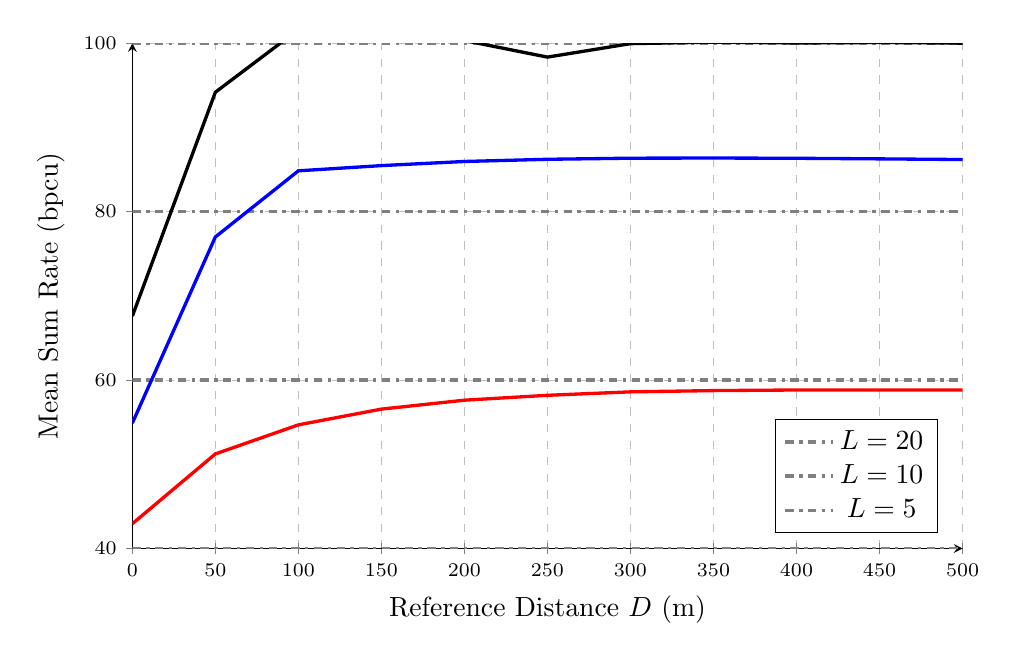
\begin{tikzpicture}
    \begin{axis}[
        width=\textwidth,
        height=8cm,
        xlabel={Reference Distance $D$ (m)},
        ylabel={Mean Sum Rate (bpcu)},
        legend pos=south east,
        xmin=0,
        xmax=500,
        ymin=40,
        ymax=100,
        ytick={40,60,...,100},
        tick label style={font=\scriptsize},
        grid=both,
        grid style=dashed,
        axis lines=left,
        enlargelimits=false,
        ]
    \addplot [very thick,dashdotted,color=gray] coordinates {(0, 100)(500, 100)};
    \addplot [very thick,dashdotted,color=gray] coordinates {(0, 80)(500, 80)};
    \addplot [very thick,dashdotted,color=gray] coordinates {(0, 60)(500, 60)};
    \addplot [very thick,dashdotted,color=gray] coordinates {(0, 40)(500, 40)};
    \addplot [very thick,color=black] table[x=D,y expr=\thisrow{sum_rate}] {
D        sum_rate
0       67.59
50      94.17
100     101.61
150     101.78
200     100.31
250     98.34
300     99.94
350     100.12
400     100.02
450     100.08
500     100.00
};
\addlegendentry{$L=20$}
\addplot [very thick,color=blue] table[x=D,y expr=\thisrow{sum_rate}] {
D        sum_rate
0       54.89
50      76.99
100     84.84
150     85.46
200     85.95
250     86.21
300     86.34
350     86.36
400     86.33
450     86.26
500     86.18
};
\addlegendentry{$L=10$}
\addplot [very thick,color=red] table[x=D,y expr=\thisrow{sum_rate}] {
D        sum_rate
0       42.94
50      51.23
100     54.68
150     56.55
200     57.61
250     58.19
300     58.60
350     58.75
400     58.82
450     58.82
500     58.82
};
\addlegendentry{$L=5$}
    \end{axis}
\end{tikzpicture}

\end{document}